\begin{activite}[Aire ou périmètre]

\begin{partie}[Au jardin]
\begin{enumerate}
 \item Sur un paquet de graines de gazon, il est écrit : « poids net 500 g pour environ 20 m\up{2} ». Que doit calculer Jean pour savoir combien de paquets de graines il doit acheter pour ensemencer son jardin rectangulaire de 25 m sur 30 m ?
 \item Jean veut entourer son jardin d'une haie d'arbustes. Le vendeur lui dit que les plants devront être espacés de 1,60 m pour obtenir une haie uniforme.
 
Que doit calculer le jardinier pour déterminer le nombre de plants à acheter ?
 \end{enumerate}
\end{partie}

\begin{partie}[À la maison]
Monsieur Louis veut poser un parquet dans la chambre de son fils. Le modèle de parquet choisi est vendu 45 CHF le m\up{2}. Il souhaite poser, tout autour de la chambre, une plinthe vendue 9 CHF le mètre. Les dimensions de la chambre sont de 3 m sur 4 m.
\begin{enumerate}
 \item Que doit‑il calculer pour déterminer le prix du parquet ?
 \item Que doit‑il calculer pour déterminer le prix des plinthes ?
 \end{enumerate}
\end{partie}

\begin{partie}
Propose plusieurs situations faisant intervenir l'\textbf{aire} ou le \textbf{périmètre}.
\end{partie}

\end{activite}

%%%%%%%%%%%%%%%%%%%%%%%%%%%%%%%%%%%%%%%%%%%%%%%%%%%%%%%%%%%%%%%%%

\begin{activite}[Comparaisons]

\begin{partie}[Quadrillage hexagonal] \label{PerimAires_act1}
\begin{minipage}[c]{0.65\linewidth}
\begin{enumerate}
 \item Détermine l'aire de chacune des figures colorées. Tu prendras 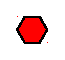
\includegraphics[width=0.5cm]{hexagone2} pour unité d'aire.
 \item Détermine le périmètre de chaque figure colorée, l'unité de longueur sera le côté d'un hexagone.
 \end{enumerate}
 \end{minipage} \hfill%
 \begin{minipage}[c]{0.3\linewidth}
  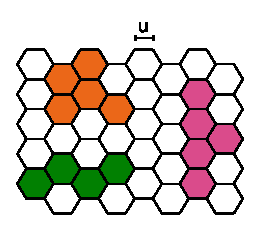
\includegraphics[width=3.7cm]{alveare}
  \end{minipage} \\
\end{partie}

\begin{partie}[Quadrillage triangulaire] \label{PerimAires_act2}
\begin{minipage}[c]{0.5\linewidth}
Mêmes questions que dans la partie \ref{PerimAires_act1}. L'unité d'aire est 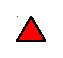
\includegraphics[width=0.45cm]{triangle} et l'unité de longueur le côté d'un triangle.
 \end{minipage} \hfill%
 \begin{minipage}[c]{0.46\linewidth}
  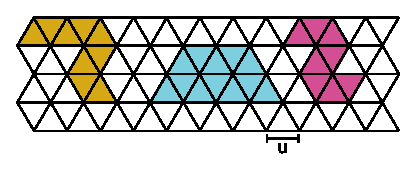
\includegraphics[width=6.2cm]{uniteU}
  \end{minipage} \\
\end{partie}

\begin{partie}
Observe les résultats des questions dans les parties \ref{PerimAires_act1} et \ref{PerimAires_act2} pour répondre aux questions suivantes :
\begin{enumerate}
 \item Les figures ayant la plus grande aire ont‑elles le plus grand périmètre ?
 \item Les figures qui ont le plus petit périmètre ont‑elles la plus petite aire ?
 \end{enumerate}
\end{partie}

\begin{partie}[À toi de jouer]
\begin{enumerate}
 \item Sur du quadrillage, trace plusieurs figures de même aire et compare leurs périmètres ;
 \item Sur du quadrillage, trace plusieurs figures de même périmètre et compare leurs aires.
 \end{enumerate}
\end{partie}

\begin{partie}
\begin{minipage}[c]{0.48\linewidth}
En t'aidant du quadrillage, détermine  approximativement l'aire de la surface délimitée par la ligne orange.
 \end{minipage} \hfill%
 \begin{minipage}[c]{0.48\linewidth}
  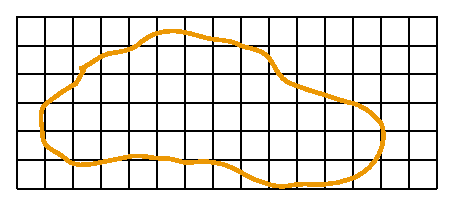
\includegraphics[width=6.8cm]{perimetre_orange}
  \end{minipage} \\
\end{partie}

\end{activite}

%%%%%%%%%%%%%%%%%%%%%%%%%%%%%%%%%%%%%%%%%%%%%%%%%%%%%%%%%%%%%%%%%

\begin{activite}[Unités d'aire]

\begin{center} 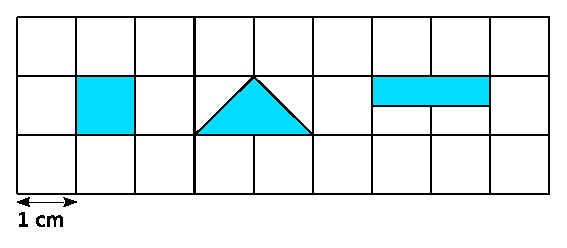
\includegraphics[width=8.5cm]{unites_aire} \end{center}

\begin{partie}
Que peux‑tu dire de l'aire des trois figures bleues ?
\end{partie}

\begin{partie}
L'aire de chacune de ces figures est la même que celle d'un carré de côté 1 cm. On dit que l'aire mesure 1 centimètre carré, on le note 1 cm\up{2}.
\begin{enumerate}
 \item Recopie et complète :
 \begin{center} \textcolor{B2}{Un centimètre carré (cm\up{2}) est la surface occupée par un carré de côté ... .} \end{center}
 \item Définis de la même façon le mètre carré, le décimètre carré, le millimètre carré et le kilomètre carré.
 \end{enumerate}
\end{partie}

\begin{partie}[Ordre de grandeur]
\begin{enumerate}
 \item Quel est l'\textbf{ordre de grandeur} de l'aire d'une page du livre ? Exprime‑la à l'aide de l'unité d'aire la mieux adaptée.
 \item Propose des objets dont l'aire est de l'ordre des unités d'aire les plus usuelles.
 \end{enumerate}
\end{partie}

\begin{partie}[Sur une feuille de papier millimétré]
\begin{enumerate}
 \item Dessine en bleu plusieurs figures dont l'aire est un centimètre carré.
 \item Dessine en rouge un carré d'aire un décimètre carré et en vert un carré d'aire un millimètre carré.
 \item Combien y a‑t‑il de centimètres carrés dans un décimètre carré ?
 \item Combien y a‑t‑il de millimètres carrés dans un centimètre carré ?
 \item Combien y a‑t‑il de millimètres carrés dans un décimètre carré ?
 \end{enumerate}
\end{partie}

\begin{partie}[Aire d'un rectangle]
\begin{minipage}[c]{0.36\linewidth}
\begin{enumerate}
 \item Détermine l'aire du rectangle bleu en centimètres carrés et en millimètres carrés ;
 \item Détermine l'aire du rectangle rouge en millimètres carrés ;
 \item Propose un moyen de déterminer l'aire du rectangle rouge en centimètres carrés.
 \end{enumerate}
 \end{minipage} \hfill%
 \begin{minipage}[c]{0.6\linewidth}
  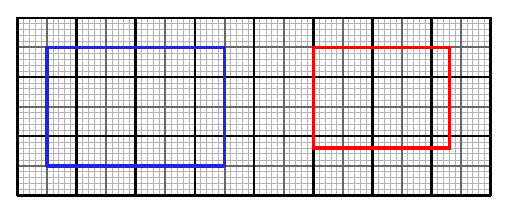
\includegraphics[width=7.6cm]{rectangles}
  \end{minipage} \\
\end{partie}

\begin{partie}
La cour d'un collège est de forme rectangulaire de 75 m sur 35 m :
\begin{enumerate}
 \item Calcule son aire en mètres carrés.
 \item Calcule son aire en décamètres carrés.
 \end{enumerate}
\end{partie}

\begin{partie}
Recherche les dimensions d'un terrain de football, de basket-ball, de tennis et calcule leurs aires respectives en mètres carrés puis en décamètres carrés.
\end{partie}

\end{activite}

%%%%%%%%%%%%%%%%%%%%%%%%%%%%%%%%%%%%%%%%%%%%%%%%%%%%%%%%%%%%%%%%%

\begin{activite}[Du rectangle au parallélogramme]

\begin{enumerate} \label{PerimAires_act3}
\item Construis, sur une feuille, un rectangle de 10 cm de long sur 4 cm de large. Repasse en rouge les longueurs et en vert les largeurs. Calcule l'aire de ce rectangle.


\item Avec un seul coup de ciseaux, découpe le rectangle fait en \ref{PerimAires_act3} puis recolle les morceaux pour obtenir un parallélogramme. Quelle est alors l’aire de ce parallélogramme ?



\item Nadir affirme : « Sur la figure suivante, les quadrilatères $TUCD$, $ABCD$ et $RSCD$ ont la même aire. ». A-t-il raison ? Justifie ta réponse.\\[0.5em]
\begin{center} 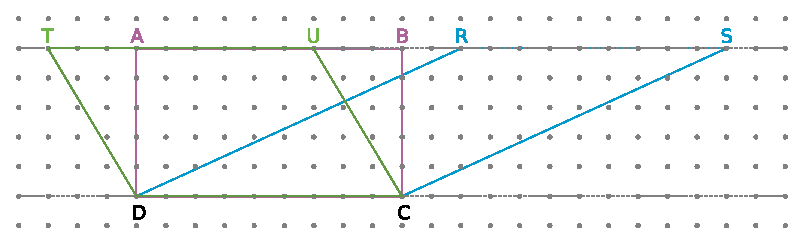
\includegraphics[width=12.4cm]{quadTAUBRS} \end{center}


\item Reproduis sur ton cahier le rectangle $ABCD$ ci-dessus puis prolonge en pointillés les droites $(BC)$ et $(AD)$. Place deux points $E$ et $F$ sur la droite $(AD)$ pour que le parallélogramme $EFBC$ ait la même aire que le rectangle $ABCD$.



\item À l'aide des questions précédentes, propose une ou plusieurs formules qui permettent de calculer l'aire du parallélogramme $EFGH$ ci-dessous.
 
\begin{center}
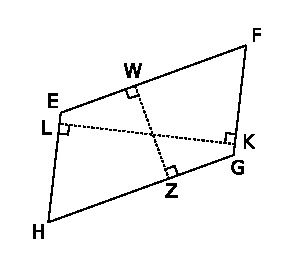
\includegraphics[width=3.6cm]{quadEWF}
\end{center}


\item Rédige une phrase pour expliquer la formule de l'aire d'un parallélogramme.
\end{enumerate}

\end{activite}

%%%%%%%%%%%%%%%%%%%%%%%%%%%%%%%%%%%%%%%%%%%%%%%%%%%%%%%%%%%%%%%%%

\begin{activite}[Perdre sa moitié]

\begin{partie}[Pour un triangle rectangle]
\begin{minipage}[c]{0.56\linewidth}
Le devant du chapeau de Jane est représenté par le croquis ci-contre.

Jeanne veut recouvrir le devant de paillettes pour le carnaval. Sur le tube de paillettes de 5 g, il est écrit qu'il faut 5 g de paillettes pour 20 cm\up{2}. Elle ne sait pas combien de tubes acheter. Elle téléphone à son amie Ipek et lui décrit la forme du chapeau.
 \end{minipage} \hfill%
 \begin{minipage}[c]{0.4\linewidth}
  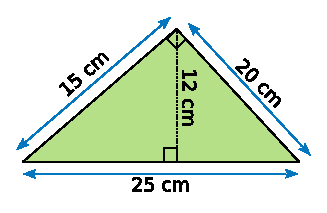
\includegraphics[width=4.8cm]{triangle_vert5}
  \end{minipage} \\
  
Ipek lui répond : « \emph{Pense à un rectangle dont l'aire est le double de ton chapeau.} »

Combien de tubes de paillettes devra acheter Jeanne ?
\end{partie}

\begin{partie}[Pour un triangle quelconque]
\begin{minipage}[c]{0.48\linewidth}
Sur la figure ci-contre, $ABCD$ est un parallélogramme de centre $O$ tel que $AB = 6$ cm et $CH = 2,5$ cm.
\begin{itemize}
 \item Calcule l'aire du parallélogramme $ABCD$.
 \item Que peux-tu observer entre les aires des triangles $ADC$ et $ABC$ ?
 \item Déduis-en l'aire du triangle $ADC$. 
 \end{itemize}
 \end{minipage} \hfill%
 \begin{minipage}[c]{0.48\linewidth}
  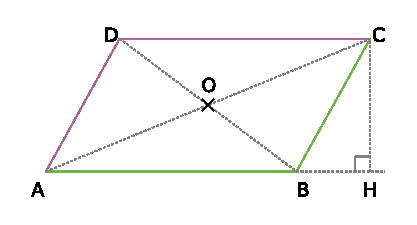
\includegraphics[width=5.5cm]{quad_rosevert}
  \end{minipage} \\[1em]
  Sur la figure ci-dessous, $ABC$ est un triangle tel que $AB = 5$ cm et $CH = 3$ cm. \\[1em]
  \begin{minipage}[c]{0.42\linewidth}
   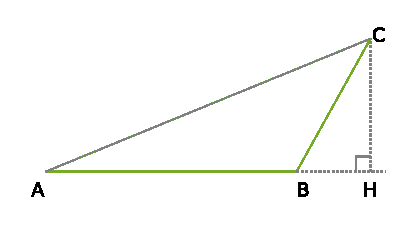
\includegraphics[width=5.4cm]{triangleABCH4} 
   \end{minipage} \hfill%
  \begin{minipage}[c]{0.54\linewidth}
  \begin{itemize}
  \item Dans le triangle $ABC$, que représente la droite $(CH)$ pour le côté $[AB]$ ?
  \item En t’inspirant de la formule de l’aire du parallélogramme, donne une formule permettant de calculer l’aire d’un triangle. 
  \item Combien y a-t-il de façons différentes de calculer l'aire d'un triangle ? Explique ta réponse.
  \end{itemize}
    \end{minipage} \\
\end{partie}

\end{activite}

%%%%%%%%%%%%%%%%%%%%%%%%%%%%%%%%%%%%%%%%%%%%%%%%%%%%%%%%%%%%%%%%%

\newpage

\begin{activite}[En découpant \ldots]

\begin{enumerate}
\item Trace un losange dont les diagonales mesurent $7,5$ cm et $9,6$ cm. Calcule son aire en le découpant de façon à obtenir une figure dont on sait calculer l'aire.

\item Halima a construit un trapèze rectangle de hauteur $4$ cm et dont les deux côtés parallèles mesurent $5$ cm et $8$ cm. Aide-la à calculer l’aire de ce trapèze.

\item Propose une méthode pour calculer l'aire d'un quadrilatère quelconque.
\end{enumerate}

\end{activite}

%%%%%%%%%%%%%%%%%%%%%%%%%%%%%%%%%%%%%%%%%%%%%%%%%%%%%%%%%%%%%%%%%

\begin{activite}[Découpages]

\begin{minipage}[c]{0.76\linewidth}
On considère un carré de côté 6 cm composé de sept polygones particuliers comme l'illustre la figure ci-contre. On sait que le segment rouge mesure $2,2$ cm en vraie grandeur.
 \end{minipage} \hfill%
 \begin{minipage}[c]{0.2\linewidth}
  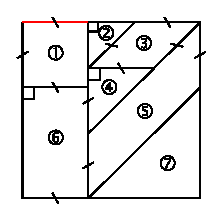
\includegraphics[width=3.1cm]{decoupage1}
  \end{minipage} \\

\begin{enumerate}
\item Précise la nature de chaque polygone puis détermine son aire.

\item Sur une feuille, construis en vraie grandeur le carré et découpe les sept pièces qui le constituent.

\item En assemblant plusieurs de ces pièces, reconstitue chacune des figures suivantes et calcule leur aire :

  \begin{colenumerate}{2}
   \item
   
   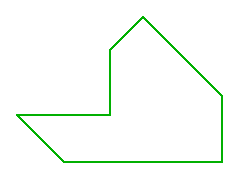
\includegraphics[width=3.3cm]{decoupage2}
   \item
   
   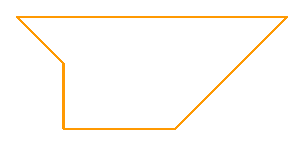
\includegraphics[width=4.4cm]{decoupage3}
   \end{colenumerate}
\end{enumerate}
\end{activite}




